\documentclass[12pt]{article}

\usepackage{sbc-template}
\usepackage{amsmath}
\usepackage{graphicx,url}

%\usepackage[brazil]{babel}   
\usepackage[utf8]{inputenc}  

     
\sloppy

\title{Travelling Salesperson Problem:\\ Handling an Intractable Problem with Approximations}

\author{Juan M. Braga F.\inst{1}}


\address{Departamento de Ciência da Computação -- Universidade Federal de Minas Gerais
  (UFMG)\\
  Av. Pres. Antônio Carlos, 6627 -- Pampulha -- Belo Horizonte -- MG -- Brazil
  \email{juanbraga@ufmg.br}
}

\begin{document} 

\maketitle

\begin{abstract}
  This paper documents the practical aspects of implementing solutions
  for the Travelling Salesperson Problem, a well-known difficult problem that requires
  exponential time for the optimal solution. Three algorithms were implemented:
  an exact solution through the branch-and-bound technique, and two other approximations,
  the Twice Around the Tree and Christofides algorithms. They were then compared in terms of
  their solution quality, execution time, and memory usage.
\end{abstract}
     
\begin{resumo} 
  Este artigo documenta os aspectos práticos da implementação de soluções
  para o Problema do Caixeiro Viajante, um problema bem conhecido e difícil que requer
  tempo exponencial para encontrar a solução ótima. Foram implementados três algoritmos:
  uma solução exata através da técnica de branch-and-bound, e duas outras aproximações,
  os algoritmos Twice Around the Tree e Christofides. Eles foram então comparados em termos de
  sua qualidade de solução, tempo de execução e uso de memória.
\end{resumo}


\section{Introducing the Travelling Salesperson Problem} \label{sec:intro}

The Travelling Salesperson Problem (TSP) is aptly described by \cite{brilliant_explanation} 

\begin{quote}
  "A salesperson needs to visit a set of cities to sell their goods. They know how 
  many cities they need to go to and the distances between each city. In what order 
  should the salesperson visit each city exactly once so that they minimize their 
  travel time and so that they end their journey in their city of origin?"
\end{quote}

The TSP is a well-known \textbf{intractable problem}, which in the context of 
algorithm complexity means that the time and/or space required to solve the problem grows 
exponentially with the size of the input, making it impractical to solve even for 
relatively small inputs.

This project documents the development of three solutions for the given problem, 
focusing on evaluating the real-world challenges associated with them, such as planning and 
optimization, making informed decisions on data structures and libraries, and 
analysing the usage of computer resources.

\section{Algorithms} \label{sec:algorithms}

The TSP problem can be conveniently modelled by a weighted graph, with the graph's 
nodes representing the cities and the edge weights specifying the distances. One benefits 
from \textbf{picturing the problem as a tree}, especially in Section~\ref{sec:optimal_explanation}.

In this project, three algorithms were implemented: an optimal solution using the \textit{Branch and Bound} technique, and two approximations, the \textit{Twice Around the Tree} and the 
\textit{Christofides} algorithms.

It must be noted that the approximation algorithms rely on the assumption that the instances of the problem obey the \textbf{triangle inequality}: in simple terms it says that no single side of a triangle can be greater than the sum of the two others (which is reasonable for most real-world applications).

\subsection{Optimal Solution: Branch and Bound} \label{sec:optimal_explanation}

As a hard problem, the most straightforward approach is the \textit{brute force} method, which involves generating all possible permutations of the cities and calculating the total distance for each permutation. However, evaluating the permutations quickly becomes impractical as the number of cities increases, and this may just be the only way to look for the optimal solution on similar problems.

To overcome this limitation, the \textit{Branch and Bound} technique provides a more efficient alternative. Instead of exploring all possible permutations, it divides the problem into smaller subproblems and makes informed decisions to discard some of these subproblems, effectively pruning the "search space".

Simply storing all paths would evidently yield a lot of data, as all possible combinations would end up stored in memory. That is why the algorithm must make smart decisions when choosing which city to visit next, which is called a \textbf{lower bound}.

This lower bound parameter is calculated by summing the total distance of the previously calculated partial paths and checking which new path to unvisited cities would be the shortest. By maintaining this metric, the \textit{Branch and Bound} algorithm can discard subproblems that will not lead to the optimal solution, and focus on the most promising paths.

Additionally, there can be made a choice of which method to traverse the "space" of 
possibilities: \textbf{best-first-search} or \textbf{depth-first-search}. The \textit{best} 
variety means that every neighbouring city will have its path calculated before a choice is 
made, which will allow the algorithm to make better-informed decisions to discard the branches, 
but will require a more memory. And secondly, the \textit{depth} variety of traversal is the 
standart search that goes deeper in the tree, which will require less space but may spend more 
time traversing the branches. As this is an expensive approach, the DFS was chosen.

The \textit{Branch and Bound} technique has a \textbf{worst-case} time complexity of $O(n!)$, 
where $n$ is the number of cities, because it may need to explore all possible permutations. 
However, effective bounding can significantly reduce the number of examined permutations, 
making it more efficient than a naive brute-force approach. The actual performance depends on 
the specific instance of the problem and the bounding technique used.

\subsection{Approximate Solution: Christofides} \label{sec:chris_explanation}

The \textit{Christofides} algorithm was built by leveraging a key insight: many of the edges on the 
optimal solution are often found on the Minimum Spanning Tree (MST) of the same graph 
\footnote{\cite{reducible_explanation}}. Therefore, as there are known relatively efficient 
algorithms for generating the MST (such as \textit{Prim's} and \textit{Kruskal's} algorithms, presented previously during DCC206 classes), it makes sense to try and make use of this fact.

To form an optimal solution, all nodes of the MST should have an even number of edges, so 
that the salesperson could enter and leave the city through exactly two edges (also known as an 
\textit{Eulerian Tour}). However, most MSTs have nodes with an odd number of edges, 
which will require more edges to be added.

The second part of the solution involves finding good edge candidates to append to these odd 
edges from the MST. Out of multiple available options, the approach used in this implementation was the minimmn-length
matching of the odd-degree nodes, which tries to find a maximum matching in a \textit{bipartite 
graph}\footnotemark with minimum total weight. In other words, it tries to find the best nodes (shortest distance) 
that connect every pair of the odd-degree nodes of the MST.

\footnotetext{A graph is bipartite if its vertices can be divided into two groups such that no two edges connect vertices from the same group.}

Combining the MST with the minimum-length matching will provide us with a very good 
approximation of the TSP's optimal solution, which can be easily constructed by
traversing this graph while taking shortcuts to avoid visiting multiple cities.

According to \cite{Johnson2003}, the \textit{Christofides} algorithm provides a better 
\textbf{worst-case} guarantee than any other currently known tour construction heuristic: a worst case ratio of 1.5, which means that the total cost of the path found is at most twice the cost of the optimal solution; 
[and] it also tends to find better tours in practice. However, computing the minimum-length 
matching on the odd-degree vertices remains the bottleneck of the algorithm.

\subsection{Approximate Solution: Twice Around the Tree} \label{sec:twice_explanation}

The \textit{Twice Around the Tree} also uses the MST to generate a solution. The idea is to generate a path by 
traversing this MST twice, once in each direction (which means cities are allowed to be visited 
more than once). This can be done by a Depth-First Search (DFS) traversal.

To improve the quality of the solution, the algorithm then tries to shortcut the 
path by adding extra edges to it. These edges are chosen in such a way as to reduce 
the overall path length. The algorithm continues to add edges until the path length 
does not change significantly.

This algorithm has a \textbf{worst-case} guarantee of 2 (also called \textit{2-approximate}), meaning 
that the total cost of the path found is at most twice the cost of the optimal solution.

One can implement an optimisation and reach an algorithm similar to the \textit{Approx-TSP-Tour} 
described by \cite{cormen}, and this approach has polynomial time: its complexity is $(number\_of\_cities)^2$.

\section{Implementation Choices, Dataset and Execution Instructions} \label{sec:implementation}

The programming language used was Python 3.12, and the program was executed 
in a Python Virtual Environment on the Ubuntu 23.10 Linux distribution, on a computer with a 
Intel Core i5-4690K processor and 8GB of RAM at 2133MHz.

The \textbf{datasets} were selected by the professor from the TSPLIB 95 \cite{dataset_lib}. They are composed of a sequence of 78 instances that gradually increase the number of nodes/cities, from 52 and up to 18512. They are 
stored in \texttt{.tsp} files with the node key and its $x$ and $y$ location in the cartesian plane. 
The graphs are to be constructed by considering that all cities are connected to all other cities, forming 
a totally connected graph. All instances are considered to respect the \texttt{triangle inequality} rule (see Section~\ref{sec:algorithms} for more information).

The chosen \textbf{data structure} for the approximate algorithms was the graph implementation 
by the \texttt{networkx} library in python \cite{networkx_docs}, as recommended by 
the professor in the project specifications. To prevent excessive use of Python loops, 
the internal \texttt{networkx} functions were also used, such as \texttt{minimum\_spanning\_tree}, 
\texttt{eulerian\_circuit} and \texttt{min\_weight\_matching}.

The \textbf{libraries} \texttt{time} and \texttt{memory\_profiler}\footnotemark were chosen to keep track of time 
and allocated memory, as they provided the most convenient interface. As mentioned before, the \texttt{networkx} library was also used. 

\footnotetext{The library to monitor memory significantly increases memory use, so the program can be run to just keep track of memory and also to collect just the other metrics.}

\textbf{Execution Instructions:}

\begin{itemize}
  \item Make sure that a compatible Python version and the libraries used (see above) are installed.
  \item Select the desired datasets to be used in the \texttt{dataset\_recipe.txt} file.
  \item Make sure the respective dataset \texttt{.tsp} files are in the \texttt{datasets/} subfolder.
  \item Choose which algorithm will be run and wether to skip memory monitoring in the \texttt{main.py} file. (Look for the \texttt{run\_algorithm\_name} boolean variables in the \texttt{main} function.)
  \item Run the code in a terminal with the following command: \texttt{python main.py} or \texttt{python3 main.py}.
  \item The results are stored as a \texttt{.csv} file within the subfolder \texttt{statistics}, named "results" and followed by a timestamp.
\end{itemize}

\section{Experiments and Discussion} \label{sec:experiments}

The qualities of each algorithm will be evaluated through four metrics: the time elapsed 
to find the solution, the amount of memory used and the quality of the solutions found 
compared to the optimal solution (see Section~\ref{sec:implementation} for information 
on the dataset and libraries used).

\subsection{Memory Use} \label{sec:exp_memory}

The first and most important aspect when dealing with exponential optimisation problems such as 
the TSP is the use of memory. To make informed decisions about all possible combinations, 
it is often necessary to store information about many or all of the previous decisions, not to 
mention storing the entire problem.

For this project, the chosen data structure implementation (Section~\ref{sec:implementation}) works by storing 
the entire graph in memory, so simply storing the dataset is the first memory bottleneck.

For the algorithms themselves, see the maximum allocated memory for each test case in Figure~\ref{fig:mem_use}.

\begin{figure}[ht]
\centering
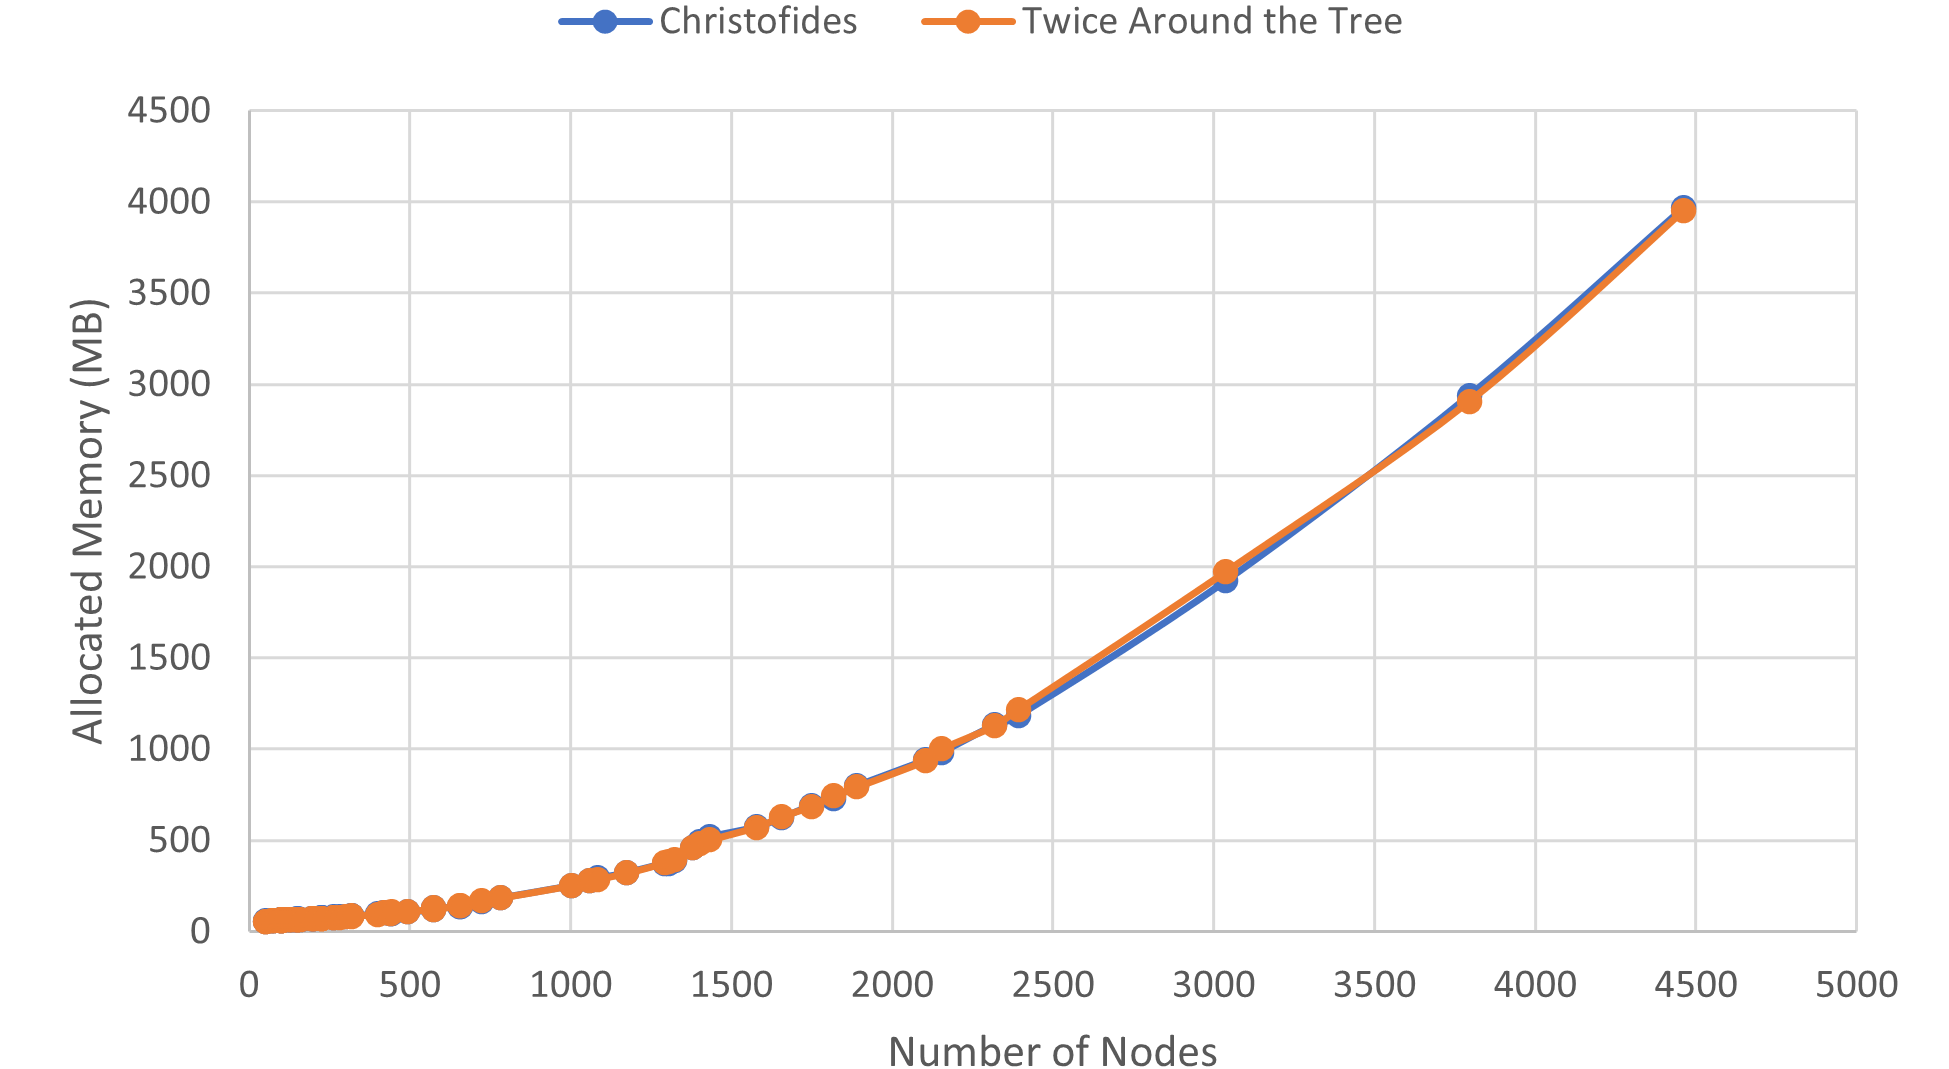
\includegraphics[height=.325\textheight]{images/memory_use_comparison.png}
\caption{Comparison of the maximum allocated memory by the \textit{Christofides} and the \textit{Twice Around the Tree} algorithms.}
\label{fig:mem_use}
\end{figure}

This first graph displays a similar memory footprint for both algorithms. However, to put things in perspective, 
we should take a look at Figure~\ref{fig:memory_behaviour}.

\begin{figure}[ht]
\centering
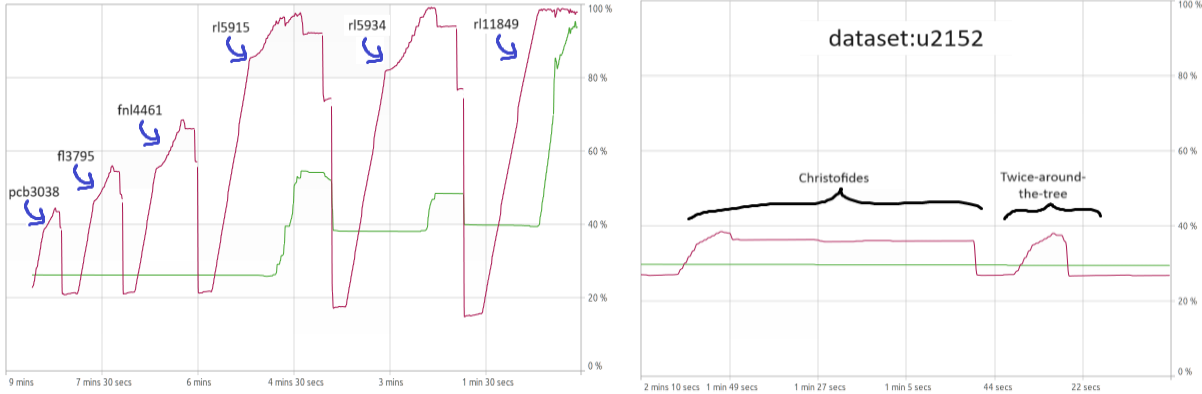
\includegraphics[width=\textwidth]{images/memory_profile_comparison.png}
\caption{(a) Memory footprint of the system during the execution of the \textit{Twice Around the Tree} algorithm on problems with increasing size. (b) Memory footprint for both \textit{Christofides} and \textit{Twice Around the Tree} algorithms, for the same instance.}
\label{fig:memory_behaviour}
\end{figure}

The first thing that must be noted it that for each algorithm there was a dataset where the allocated memory surpassed 
the available RAM capacity, and storage in the \texttt{swap}\footnotemark file was triggered. This can be seen starting from the the dataset \texttt{rl5915} execution with the \textit{Twice Around the Tree}, 
in Figure~\ref{fig:memory_behaviour} (a). This behaviour is similar in the \textit{Christofides} algorithm.

\footnotetext{Swap or Page file is a section of a hard drive used as a temporary location to store information 
when the computer's RAM (random-access memory) is fully utilized. It has significantly slower speeds when 
compared to the RAM.}

Secondly, from the \texttt{rl11849} dataset onward the computer did not have enough memory and swap to 
even build the graph in the executions (See Figure~\ref{fig:memory_behaviour} 
(a)), causing the computer to crash\footnotemark. 
(As the use of the \textit{memory\_profiler} gives us a significantly larger memory footprint, executing the smaller 
\texttt{rl5915} and \texttt{rl5934} datasets with it was also not possible.)

\footnotetext{Even though the computer crashed when reaching maximum RAM + swap usage, the student noticed that running 
the same instances in Microsoft Windows did not cause a crash. Sadly, the available Windows machine was underpowered and so this option was ignored.}

The Figure~\ref{fig:memory_behaviour} (b) also corroborates the idea of how their memory footprint is similar 
(using a small dataset to fit the execution time of the \textit{Christofides} algorithm).

Lastly, the student was not able to implement a useful \textit{Branch and Bound} solution to compare with the approximations. 
Every attempt, either in Python or C++, has caused an explosive use of memory, crashing the computer 
even for the smallest dataset. The student is forced to conclude that trying to solve this problem with this 
approach is not practical in the absolute sense, although there may be trickier and more efficient ways of 
implementing a somewhat-viable solution. He is, however, assured that choosing the \textit{Depth-First-Search} was the right intuition.

\subsection{Solution Quality} \label{sec:exp_quality}

The graph of the Figure~\ref{fig:quality_ratio} shows the ratio $\frac{Approximate Solution}{Optimial Solution}$.

\begin{figure}[ht]
\centering
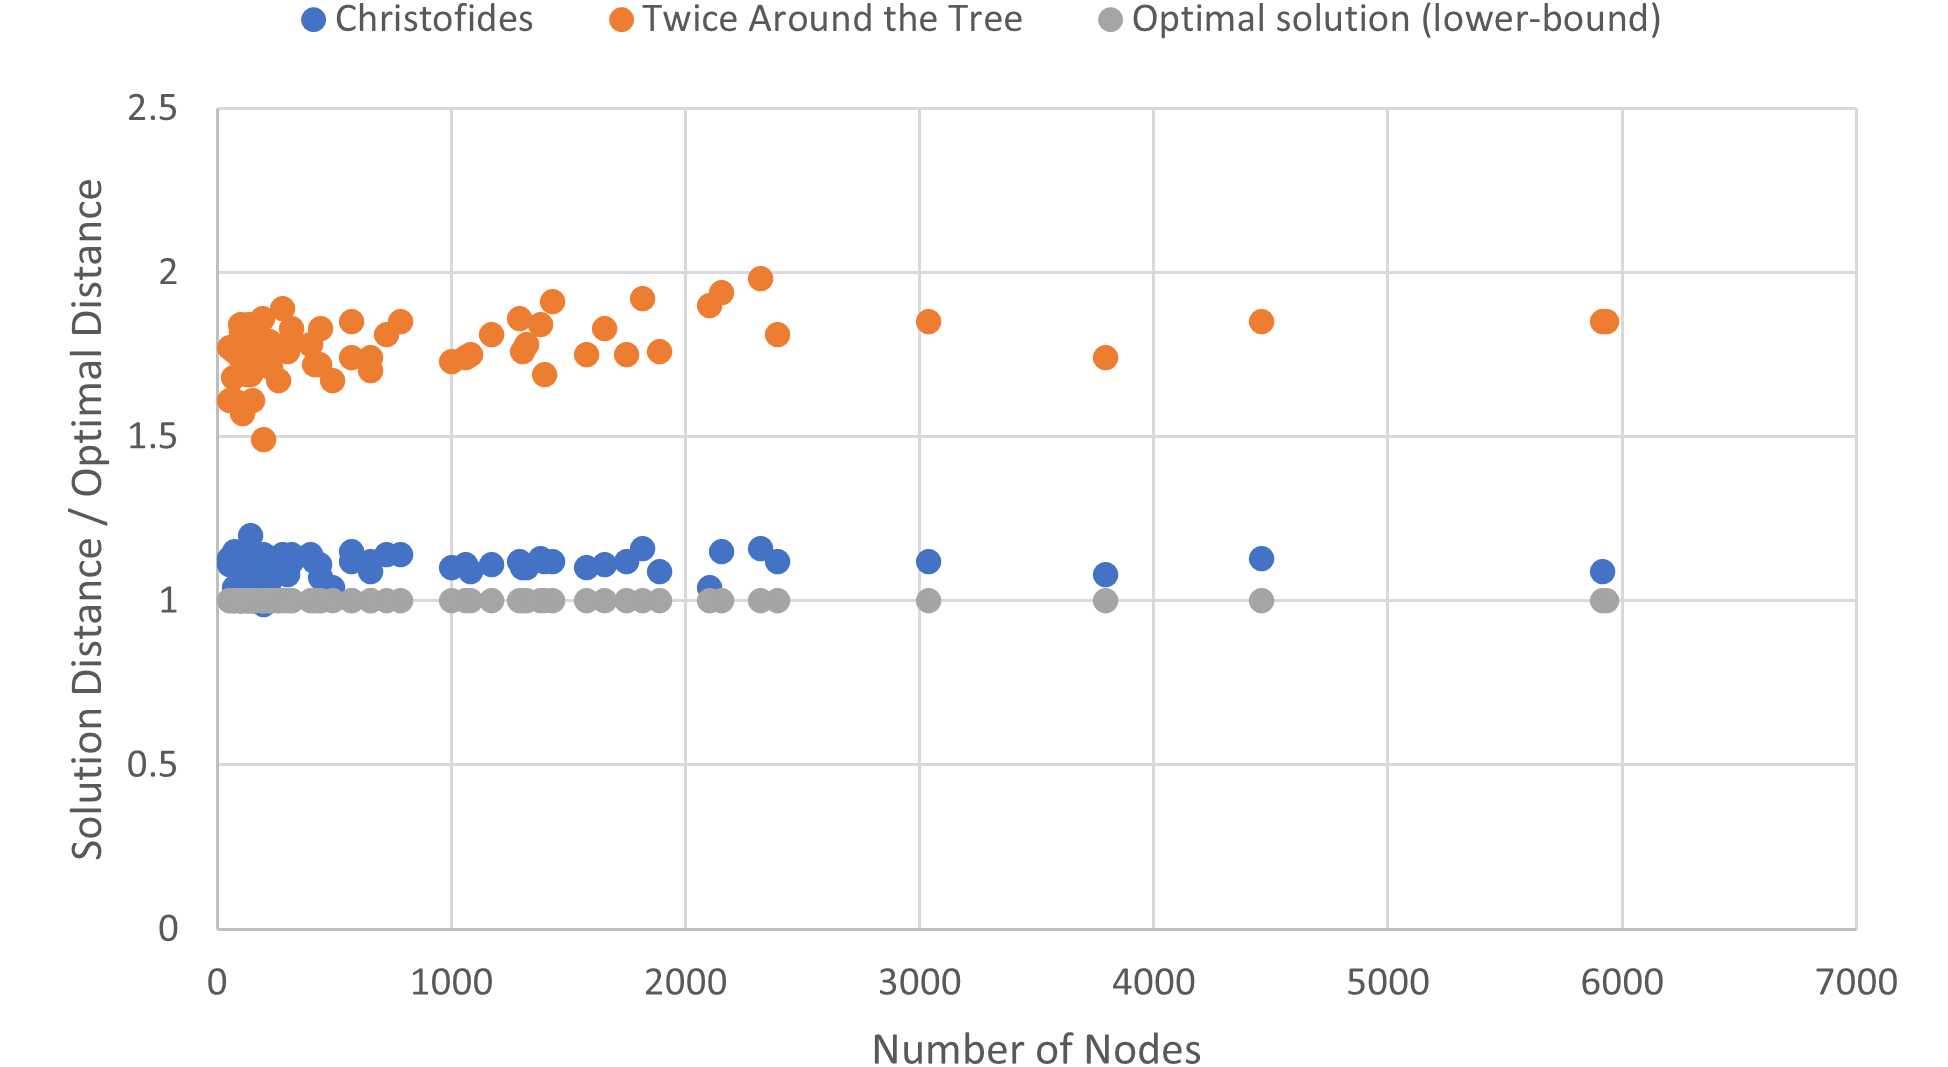
\includegraphics[height=.325\textheight]{images/quality_ratio.png}
\caption{Chart comparing the quality of the approximate and optimal solutions.}
\label{fig:quality_ratio}
\end{figure}

The \textit{Twice Around the Tree} stays consistently below the expected theoretical worst case (Section~\ref{sec:twice_explanation}) of 
twice the optimal solution, and the \textit{Christofides} solutions find paths that are consistently better and closer to it, 
also keeping the tight 1.5 quality ratio specified in Section~\ref{sec:chris_explanation}.

\subsection{Execution Time} \label{sec:exp_time}

The execution time of the algorithms can be compared with the following Figure~\ref{fig:exec_time}.

\begin{figure}[ht]
\centering
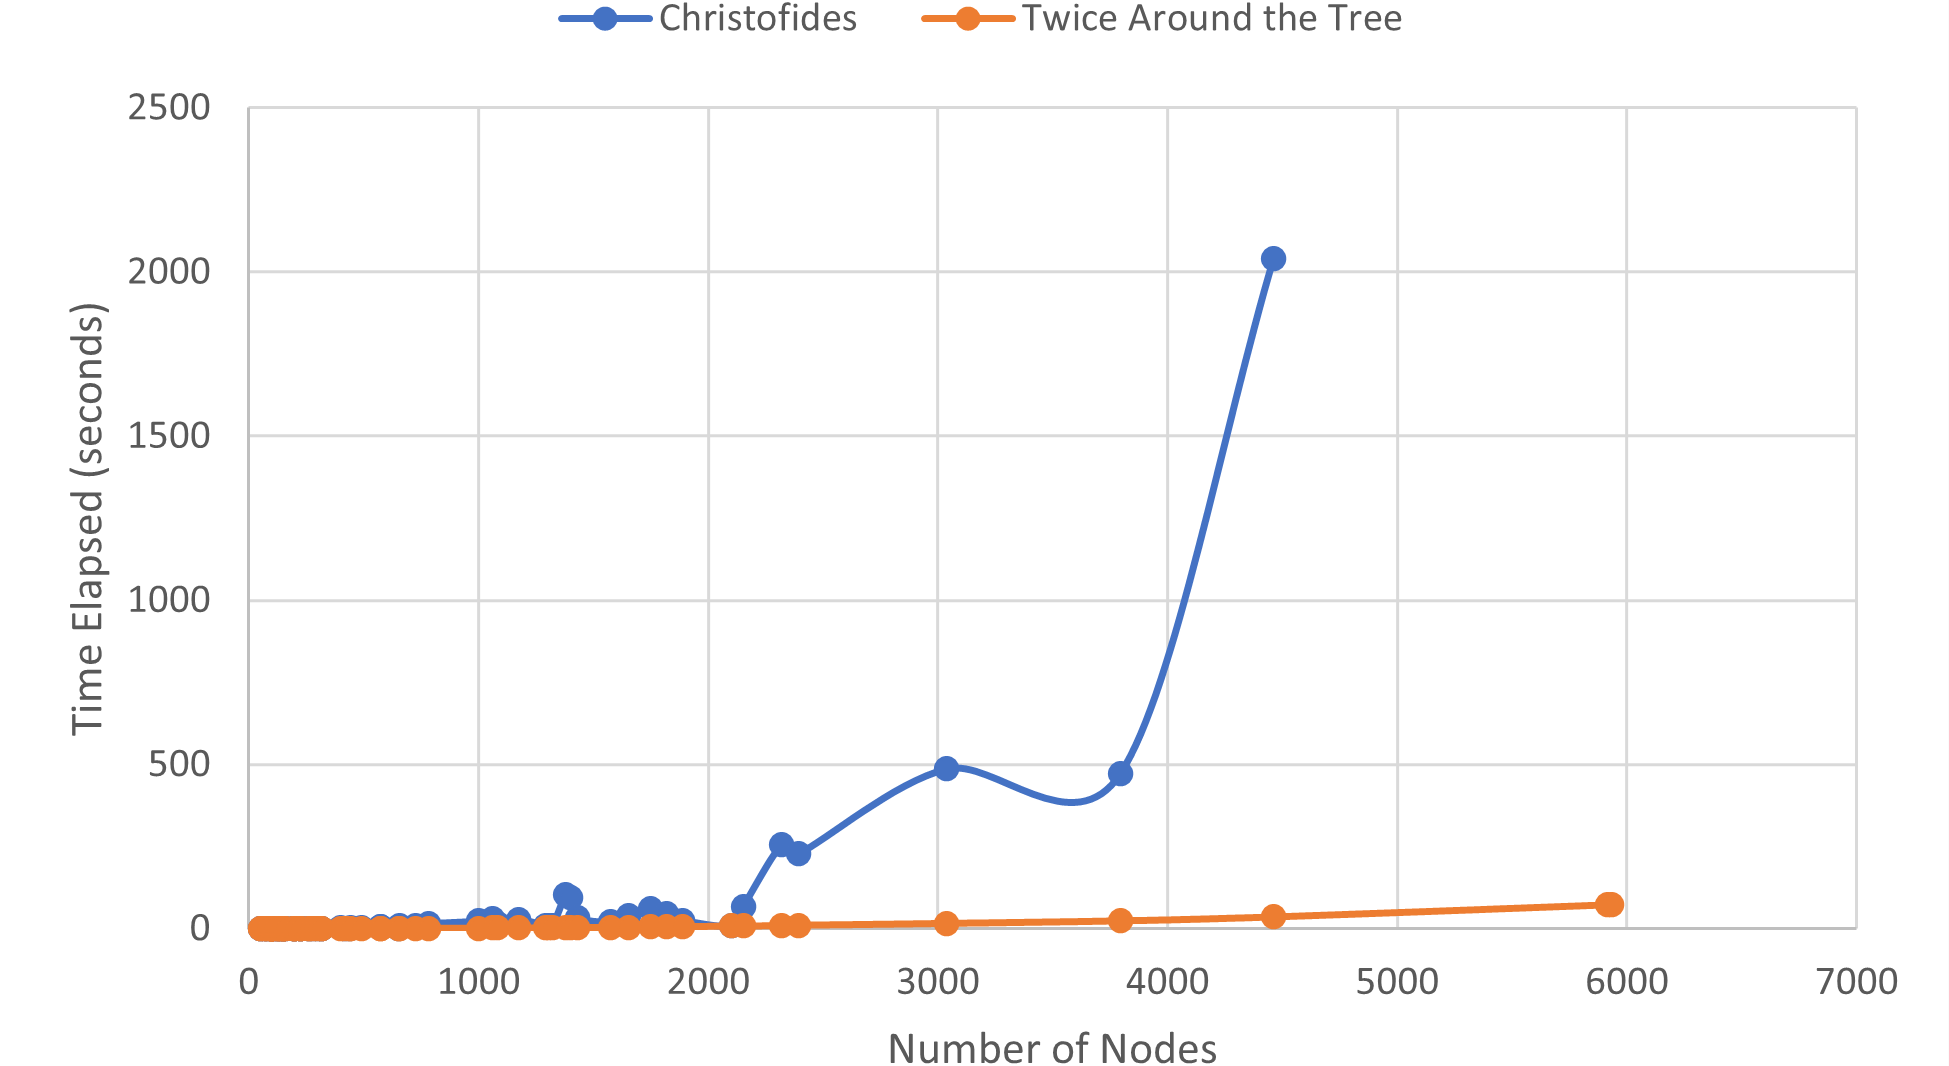
\includegraphics[height=.325\textheight]{images/execution_time_comparison.png}
\caption{Chart comparing the time elapsed between the \textit{Christofides} and the \textit{Twice Around the Tree} algorithms.}
\label{fig:exec_time}
\end{figure}

The \textit{Christofides} algorithm takes significantly longer to run when compared to the \textit{Twice Around the Tree} algorithm. 
In fact, it appears to form an exponential growth. However, as diagnosed in Section~\ref{sec:exp_memory}, the algorithms exceeded the available RAM memory, so this claim must be put into perspective.
This fact can explain why the \texttt{fnl4461} case has shown such a drastic increase in execution time: the use 
of swap memory has slowed it down, and from this point onward the graph will not display its ideal behaviour. In 
other words, this does not constitute as evidence that the \textit{Christofides} algorithm is exponential 
(See Section~\ref{sec:chris_explanation}).

This perfectly illustrates how difficult of a problem it is to optimise exponential algorithms, even for relatively 
small cases. The \textit{Twice Around the Tree}, although having a much worse quality then the \textit{Christofides}, is 
significantly faster and should provide good-enough answers for the right situations.

\section{Conclusions} \label{sec:conclusions}

Implementing the algorithms provided valuable insights into the real-world aspects of solving the TSP and likely other hard problems. 
It demonstrated the trade-offs between solution quality, execution time, and memory requirements, 
and highlighted the limitations of exponential algorithms, as the \textit{Branch and Bound} technique quickly becomes intractable for even relatively small instances of the problem.

For the approximations, both had very similar memory requirements, but the Cristofides algorithm consistently outperformed the \textit{Twice Around the Tree} 
algorithm in terms of solution quality, maintaining a tight 1.5 quality ratio with the optimal 
solution. However, it is significantly slower. The \textit{Twice Around the Tree} algorithm, on the other hand, 
offers a reasonable trade-off between solution quality and execution time.

The results suggest that the \textit{Twice Around the Tree} algorithm is a good choice for practical applications of the 
TSP, as it provides a reasonable balance between quality and efficiency. The \textit{Christofides} algorithm can be used 
when a high-quality solution is required, but it is important to be aware of its computational limitations.

\bibliographystyle{sbc}
\bibliography{sbc-template}

\end{document}
